\documentclass[crop,tikz]{standalone}
\usepackage[english]{babel}
\usepackage{amsmath,amssymb}
\usepackage{bbm}
\usepackage{graphicx}
\usepackage{tikz}
\usepackage{xcolor}

\usetikzlibrary{arrows, positioning, shapes}
\tikzset{
	%Define standard arrow tip
	>=stealth',
	% Define arrow style
	pil/.style={
		->,
		thick,
		shorten <=2pt,
		shorten >=2pt
	},
	map/.style={
		|->,
		thick,
		shorten <=2pt,
		shorten >=2pt
	}
}

\definecolor{tabblue}{HTML}{1f77b4}
\definecolor{taborange}{HTML}{ff7f0e}
\definecolor{tabgreen}{HTML}{2ca02c}
\definecolor{tabred}{HTML}{d62728}
\definecolor{tabpurple}{HTML}{9467bd}
\definecolor{tabbrown}{HTML}{8c564b}
\definecolor{tabpink}{HTML}{e377c2}
\definecolor{tabgray}{HTML}{7f7f7f}
\definecolor{tabolive}{HTML}{bcbd22}
\definecolor{tabcyan}{HTML}{17becf}




\begin{document}

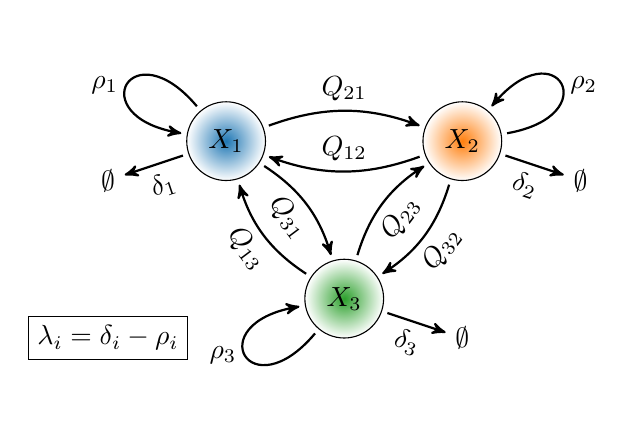
\begin{tikzpicture}
\node[circle, draw, black, inner color=tabblue, outer color=white, inner sep=0, minimum size=10mm] at (1,3.5) (X1) {$X_1$};
\node[circle, draw, black, inner color=taborange, outer color=white, inner sep=0, minimum size=10mm] at (4,3.5) (X2) {$X_2$};
\node[circle, draw, black, inner color=tabgreen, outer color=white, inner sep=0, minimum size=10mm] at (2.5,1.5) (X3) {$X_3$};

\node at (-0.5, 3) (null1) {$\emptyset$};
\node at (5.5, 3) (null2) {$\emptyset$};
\node at (4.0, 1.0) (null3) {$\emptyset$};

\node[rectangle, draw] at (-0.5, 1.0) (eqn) {$\lambda_i = \delta_i - \rho_i$};
% proliferation

\path[pil] (X1) edge[loop left, in=170, out=130, looseness=10] node (p1) {$\rho_1$} (X1);
\path[pil] (X2) edge[loop right, in=50, out=10, looseness=10] node (p2) {$\rho_2$} (X2);
\path[pil] (X3) edge[loop left, in=-170, out=-130, looseness=10] node (p3) {$\rho_3$} (X3);

% death

\path[thick, shorten <=2pt, ->] (X1) edge node[sloped, below] (d1) {$\delta_1$} (null1);
\path[thick, shorten <=2pt, ->] (X2) edge node[sloped, below] (d1) {$\delta_2$} (null2);
\path[thick, shorten <=2pt, ->] (X3) edge node[sloped, below] (d1) {$\delta_3$} (null3);

% differentiation

\path[pil] (X1) edge[bend left=20] node[above] (Q21) {$Q_{21}$} (X2);
\path[pil] (X2) edge[bend left=20] node[above] (Q12) {$Q_{12}$} (X1);

\path[pil] (X1) edge[bend left=20] node[sloped, below] (Q31) {$Q_{31}$} (X3);
\path[pil] (X3) edge[bend left=20] node[sloped, below] (Q13) {$Q_{13}$} (X1);

\path[pil] (X2) edge[bend left=20] node[sloped, below] (Q32) {$Q_{32}$} (X3);
\path[pil] (X3) edge[bend left=20] node[sloped, below] (Q23) {$Q_{23}$} (X2);



\end{tikzpicture}


\end{document}